\section{CT, DT Sampling}
\begin{itemize}
	\item The idea is to take a signal which is continuous \( x(t) \) and convert it into a discrete
		number of samples:
		\[
		x(t) \to \{x(nT)\}, n \in \Z
		\] 
		Basically, we just get the values of \( x(t) \) at some uniform rate. The sampling frequency 
		(or sampling rate) \( f_s = 1 / T \), or \( \omega_s = 2\pi / T \), where \( T \) is the 
		sampling period (the time between samples). If the sampling rate is 1Hz, then it means that we are 
		sampling 1 value per second.  
	\item There are multiple ways of representing samples. One way is to represent them as a continuous-time 
		signal, but we now use the property of delta function:
		\[
		x_p(t) = \sum_{n=-\infty}^{\infty} x(nT) \delta(t - nT)
		\] 
		\question{Deosn't the delta function only \textit{integrate} to 1, and not sum to 1?}.

		\answer{Probably some abuse of notation here. That said, notice that \( x_p(t) \) is zero when 
		\( t \) is not a multple of \( nT \), which is the behavior we want.}

		We can also 
		represent it just as a discrete time signal:
		\[
			x_d[n] = x(nT)
		\] 
	\item For discrete-time signals, we can define a sampling function
		\[
			p[n] = \sum_{k=-\infty}^{\infty} \delta[n - kN]
		\] 
		and we get:
		\[
			x_p[n] = x[n] p[n] = \sum_{k=-\infty}^{\infty} x[kN] \delta[n - kN]
		\] 
		We change \( x[n] \) into \( x[kN] \) because the delta function only filters for \( n = kN \) for some 
		multiple of \( k \) anyways, so we can just treat it as \( x[kN] \) because those are the only terms 
		we hope to keep. So as a diagram:
		\begin{center}
			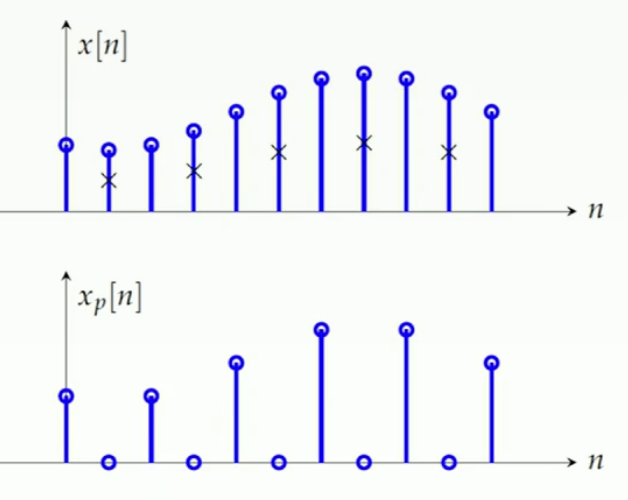
\includegraphics[scale=0.8]{discreteSample.png}
		\end{center}
	\item Just like the discrete time \( p[n] \), we can define a unit Shah function:
		\[
			\mathrm{III}(t) = \sum_{n=-\infty}^{\infty} \delta(t - n)
		\] 
		basically this is an infinite train of delta functions at \( n = 1, 2, 3, \dots \). Now if we wanted 
		to extend this into a delta train that isn't integrally spaced, we can introduce a scaling factor:
		\[
		\text{III}(t) = \sum_{n=-\infty}^{\infty} \delta\left( \frac{t}{T} - n \right) = T
		\sum_{n=-\infty}^{\infty} \delta(t - nT)
		\] 
		this usees the property taht \( \delta(at) = \frac{1}{|a|}\delta(t)  \). Therefore, we get:
		\[
		\frac{1}{T}\text{III}\left( (\frac{t}{T} \right) = \sum_{n=-\infty}^{\infty} \delta(t - nT)
		\] 
		Now, given the form of \( x_p(t)  \) that we had earlier:
		\[
		x_p(t) = \sum_{n=-\infty}^{\infty} x(nT) \delta(t - nT) = x(t) \frac{1}{T}\text{III}\left( \frac{t}{T} \right) 
		= x(t) f_s \text{III}(tf_s)
		\] 
		\comment{remember that when \( x(t) \) goes into the shah function it actually beocmes 
		\( x(nT) \) for the same reason we looked at earlier.}

		In general, sampling is basically just multiplication by a Shah function. 
\end{itemize}
\subsection{Nyquiest Theorem}
\begin{itemize}
	\item Aims to answer: can we faithfully represent a continuous time signal with a set of discrete time signals, 
		without the loss of information? Or rather, how many samples do we need to represent a CT signal into a 
		discrete signal without loss of information? 
	\item This technique is called \textit{interpolation}
	\item The simplest way to reconstruct this signal is called a \textit{zero-order hold} interpolation. Basically, 
		if \( x(t)  \) is the CT signal and \( x_0(t) \) is our sampled signal, then between 
		every sampled value, we just ``hold" the value in place at \( x_0(nT) \) until we reach the next point. 

		This system is LTI: first of all, it's linear since we just sum over the two signals for the hold, and it's 
		time invariant becuase none of the functions actually care where the signal starts. 
	\item It basically just looked like a complicated step function. 
	\item Mathematically, we'd represent this as:
		\[
		x_0(t) = x_p(t)* h_0(t)
		\] 
	\item We can also \textit{first order hold}, or also called a linear iterpolation. Here, we just join 
		two sampling points linearly together. 

		It is also LTI, for the same reasons as the zero order hold. Because it's LTI, we can write it as 
		some convolution of \( x(t) \) and an impulse response \( h_1(t) \):
		\[
		x_1(t) = x_p(t) * h_1(t) 
		\] 
		Here, \( h_1(t) \) looks like a triangular function. 
\end{itemize}
\subsection{Fourier Transforms of Sampling}
\begin{itemize}
	\item Let's start with the definition of \( x_p(t) \):
		\[
		x_p(t) = x(t) \frac{1}{T}\text{III}\left( \frac{t}{T} \right) 
		\] 
		we can take the Fourier transform of this signal and uncover the underlying frequencies:
		\[
		\mathcal F \{x_p(t)\}  = \mathcal F \{x(t) \frac{1}{T} \text{III}\left( \frac{t}{T} \right) \} 
		= \mathcal F \{x(t)\}  * \mathcal F \left\{ \frac{1}{T}\text{III}\left( \frac{t}{T} \right)  \right\} 
		\] 
		The first term gives us \( X(\omega) \), and for the second term:
		\[
		\mathcal F \left\{ \frac{1}{T}\text{III}\left( \frac{t}{T} \right)  \right\} = \frac{1}{T} T\text{III}(Tf)
		= \text{III}(Tf)
		\] 
		this property comes from \textit{time scaling}. So we can write this as:
		\[
		\frac{1}{T}\sum_{n=-\infty}^{\infty} \delta\left( f - \frac{n}{T} \right)  = f_s
		\sum_{n=-\infty}^{\infty} \delta(f - nf_s)
		\] 
		\question{Shouldn't the delta functions Fourier transform into complex exponentials?}

	\item So in general, 
		\[
			\mathcal F \{x_p(t)\} = X(f) * \text{III}(Tf)  = f_s \sum_{n=-\infty}^{\infty} X(f) * \delta(f - nf_s)
			= f_s \sum_{n=-\infty}^{\infty} X(f - nf_s)
		\]
	\item In terms of angular frequency, we have:
		\[
		\mathcal F \{x_p(t)\}  = X_p(\omega) = \sum_{n=-\infty}^{\infty} x(nT) e^{-j \omega T n}
		\] 
	\item We can do a similar analysis with \( x_d[n] = x(nT) \). We'll let \( \omega \) be the angular frequency 
		of CT signal, and let \( \omega_d \) be the angular frequency of our DT signal. Therefore:
		\[
			\mathcal F \{x_d[n]\}  = X_d(e^{j \omega_d}) = \sum_{n=-\infty}^{\infty} x_d[n] e^{-j \omega_d n}
			= \sum_{n=-\infty}^{\infty} x(nT) e^{-j \omega_d n}
		\] 
		Recalling the formula from the earlier bullet point and \( X_p(\omega) = X_d(e^{j \omega_d} \) (since 
		they're calculating the Fourier transform of the same signal \( x \)), then we have the relationship
		that \( \omega_d = \omega T \)
	\item We can go further: we know that the relatinoship between \( X_p(\omega)  \) and 
		\( X_d(e^{j \omega_d}) \), so we have:
		\[
		X_d(e^{j \omega_d}) = \frac{1}{T}\sum_{n=-\infty}^{\infty} X(\omega - n \omega_s) 
		= \frac{1}{T}\sum_{n=-\infty}^{\infty} X(\omega T - n \omega_s T) = \frac{1}{T}\sum_{n=-\infty}^{\infty} 
		X(\omega_d - 2 \pi n)
		\] 
\end{itemize}
